\section{\textsc{Coleslaw Salad}}

\subsection*{Ingredients for 2 portions:}

\begin{tabular}{p{7.5cm} p{7.5cm}}
	& \\
	\sfrac{1}{2} cabbage & 1 carrot \\
	1 onion & \sfrac{1}{2}ts pepper \\
	\sfrac{1}{2}ts salt & 1ts paprika \\
	4ts white wine vinegar & 2ts mustard \\
	125g mayonnaise & 65g sugar \\
	60ml milk & 60ml buttermilk \\
	6ts lemon juice &
\end{tabular}

\subsection*{Serving suggestion:}

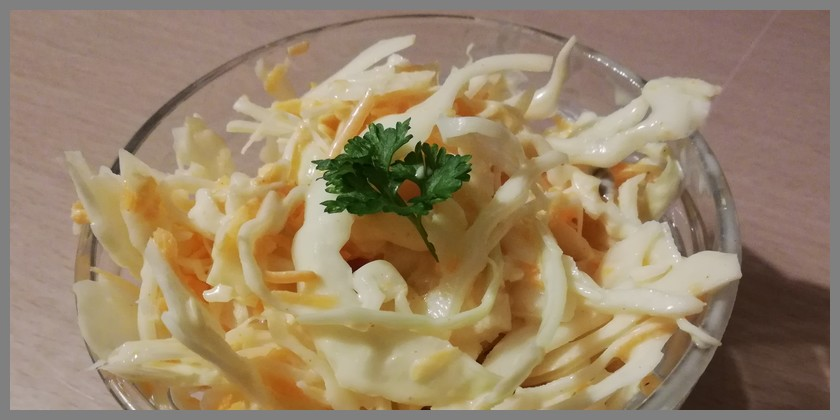
\includegraphics[width=\textwidth]{img/coleslawsalad.jpg} \cite{uskrautsalat}

\subsection*{How it's done:}
\begin{tabular}{p{15cm}}
	\\
  Cut the cabbage, the carrot and the onion in small strips (= Julienne).\\
  Now you mix the vegetables in a big bowl.\\
  After that you put the other ingredient into another bowl and mix it too.\\
  You put the dressing over the mix of the vegetables.\\
  Let the mixture pass for eight to ten hours.\\
  Before you serve it, stir it a little bit.
\end{tabular}
